\documentclass[12pt,a4paper]{article}
\usepackage{fontspec}
\usepackage[polish]{babel}
\usepackage[a4paper,margin=2.5cm]{geometry}
\usepackage{setspace}
\setstretch{1.3}
\usepackage{graphicx}
\usepackage{booktabs}
\usepackage{tabularx}
\usepackage{amsmath}
\usepackage{float}
\usepackage{caption}
\usepackage{subcaption}
\usepackage{xcolor}
\usepackage{listings}
\usepackage{enumitem}
\usepackage[hidelinks]{hyperref}
\usepackage{xurl}

\graphicspath{{img/}}
\setlength{\emergencystretch}{3em}
\captionsetup{labelsep=colon,font={small,stretch=1}}
\captionsetup[table]{position=top}

\lstset{
  language=Python,
  basicstyle=\ttfamily\footnotesize\setstretch{1},
  keywordstyle=\color{teal!70!black},
  commentstyle=\color{black!55}\itshape,
  stringstyle=\color{red!65!black},
  showstringspaces=false,
  breaklines=true,
  frame=single,
  rulecolor=\color{black},
  framesep=4pt,
  xleftmargin=4pt,
  xrightmargin=4pt,
  aboveskip=6pt,
  belowskip=10pt,
}

\newcommand{\przedmiot}{Urządzenia peryferyjne}
\newcommand{\termin}{poniedziałek 23.11.2026 grupa 8.00}
\newcommand{\temat}{Kamery cyfrowe}

\newcommand{\stronatytulowa}[1]{%
  \begin{titlepage}
    \centering
    \vspace*{1.2cm}
    \colorbox{black!4}{\parbox{3.6cm}{\centering\vspace{6pt}%
      
\includegraphics[width=2.9cm]{pwr_logo_bw.png}\\[4pt]
      {\sffamily\large\setstretch{1}Politechnika\\Wrocławska\par}\vspace{6pt}}}\par
    \vspace{2.8cm}
    {\large\textsc{\przedmiot}\par}
    \vspace{0.5cm}
    {\textsc{\termin}\par}
    \vspace{1.2cm}
    \rule{\linewidth}{1pt}\par
    \vspace{0.5cm}
    {\LARGE\bfseries\setstretch{1}\temat\\#1\par}
    \vspace{0.4cm}
    \rule{\linewidth}{1pt}\par
    \vspace{0.6cm}
    \begin{minipage}[t]{0.48\textwidth}
      \raggedright\setstretch{1.25}
      \emph{Autorzy:}\\
      Iga \textsc{Wolanin} 281203\\
      Adam \textsc{Korwin} 284455
    \end{minipage}\hfill
    \begin{minipage}[t]{0.48\textwidth}
      \raggedleft\setstretch{1.25}
      \vspace{0.3cm}
      \emph{Prowadzący:}\\
      dr inż. Dominik \textsc{Żelazny}
    \end{minipage}
    \vfill
  \end{titlepage}
}


\begin{document}
\stronatytulowa{Sprawozdanie}

\section{Cel ćwiczenia}
Celem ćwiczenia było zapoznanie się z budową i zasadą działania kamer cyfrowych (matryce
światłoczułe, odwzorowanie kolorów, parametry obrazu) oraz napisanie programu obsługującego
kamery USB. Zgodnie z poleceniem prowadzącego program miał umożliwiać wybór jednej z podłączonych
kamer, wybór jakości obrazu (rozdzielczości pracy kamery) oraz zmianę nasycenia barw, a także
wykonywanie zdjęć i nagrywanie filmów zapisywanych w standardowych formatach. Zadaniem dodatkowym
na ocenę wyższą, zrealizowanym w ramach ćwiczenia, było wykrywanie ruchu w obrazie z kamery.

\section{Wprowadzenie teoretyczne}
\subsection{Matryce światłoczułe}
Podstawowym elementem kamery cyfrowej jest matryca, czyli płytka krzemowa z siatką fotodiod
(pikseli). Foton padający na fotodiodę wybija elektron (zjawisko fotoelektryczne wewnętrzne), więc
ładunek zgromadzony w pikselu w czasie naświetlania jest proporcjonalny do natężenia światła.
Matryce różnią się sposobem odczytu tego ładunku (tabela~\ref{tab:matryce}).

\begin{itemize}
  \item \textbf{CCD} (\emph{Charge-Coupled Device}) -- ładunki są przesuwane rząd po rzędzie,
    jak w rejestrze przesuwnym, do jednego wzmacniacza i przetwornika na krawędzi matrycy.
    Wszystkie piksele przechodzą przez ten sam tor odczytu, dlatego obraz jest jednorodny
    i mało zaszumiony. Wadą jest większy pobór mocy, wolniejszy odczyt i wyższy koszt.
  \item \textbf{CMOS} (\emph{Complementary Metal-Oxide-Semiconductor}, matryca APS) -- każdy piksel
    ma własny wzmacniacz (3--4 tranzystory), a przetworniki analogowo-cyfrowe są zwykle na tej
    samej płytce. Piksele można odczytywać wybiórczo, matryca pobiera mało energii i jest tania
    w produkcji. Odczyt odbywa się zwykle wierszami (\emph{rolling shutter}), co przy szybkim ruchu
    zniekształca obraz. Matryce CMOS są stosowane w niemal wszystkich kamerach internetowych
    i telefonach, w tym w kamerach użytych w ćwiczeniu.
  \item \textbf{HAD CCD} (\emph{Hole-Accumulation Diode}) -- odmiana CCD firmy Sony, w której na
    powierzchni fotodiody dodano warstwę typu p$^+$. Warstwa ta ogranicza prąd ciemny, czyli ładunek
    powstający bez światła, a więc zmniejsza szum. W wersji Super HAD nad pikselami dodano
    mikrosoczewki skupiające światło na fotodiodzie.
\end{itemize}

\begin{table}[H]
  \centering
  \caption{Porównanie matryc CCD i CMOS}
  \label{tab:matryce}
  \begin{tabularx}{\textwidth}{lXX}
    \toprule
    Cecha & CCD & CMOS \\
    \midrule
    odczyt ładunku & przesuw do jednego wzmacniacza & wzmacniacz w każdym pikselu \\
    szum, jednorodność & niski szum, duża jednorodność & większy szum stały (różne wzmacniacze) \\
    pobór mocy & duży & mały \\
    szybkość odczytu & mniejsza & większa, możliwy odczyt fragmentu \\
    migawka & zwykle globalna & zwykle wierszowa (\emph{rolling shutter}) \\
    koszt & wyższy & niższy (standardowy proces CMOS) \\
    \bottomrule
  \end{tabularx}
\end{table}

\textbf{Rozdzielczość} matrycy to liczba pikseli, np.\ $1280\times720 = 921\,600$ pikseli
(0,92 Mpx) lub $1920\times1080 \approx 2{,}07$ Mpx. \textbf{Wymiar} matrycy podaje się często
w calach, np.\ 1/4'' lub 1/2,3''. Oznaczenie to pochodzi od lamp analizujących i nie jest
przekątną matrycy; przekątna wynosi około 2/3 tej wartości (dla 1/2,3'' około 7,7\,mm). Przy
tej samej liczbie pikseli większa matryca ma większe piksele, które zbierają więcej światła,
więc dają mniej szumu. Kamery internetowe mają małe matryce (ok.\ 1/4''), dlatego przy słabym
świetle ich obraz szybko staje się zaszumiony.

\subsection{Kolory cyfrowe}
Fotodioda mierzy tylko natężenie światła, a nie jego barwę. Aby uzyskać obraz kolorowy, nad
pikselami umieszcza się mozaikę filtrów barwnych, najczęściej \textbf{filtr Bayera}: w każdym
bloku $2\times2$ są dwa filtry zielone, jeden czerwony i jeden niebieski (układ RGGB). Zielonych
jest dwa razy więcej, ponieważ oko jest najbardziej czułe na tę barwę. Każdy piksel mierzy więc
tylko jedną składową, a dwie pozostałe są wyznaczane z sąsiednich pikseli. Proces ten nazywa się
\textbf{demozaikowaniem}. Najprostsza metoda to interpolacja dwuliniowa, np.\ składowa zielona
w pikselu czerwonym to średnia czterech sąsiednich pikseli zielonych:
\begin{equation}
  G(x,y) = \tfrac{1}{4}\left[G(x-1,y) + G(x+1,y) + G(x,y-1) + G(x,y+1)\right].
\end{equation}
Lepsze metody uwzględniają kierunek krawędzi, bo zwykła interpolacja daje na ostrych krawędziach
kolorowe obwódki i mory. Demozaikowanie wykonuje procesor kamery, więc program otrzymuje gotowe
piksele RGB (w OpenCV w kolejności BGR).

\textbf{Balans bieli} kompensuje barwę oświetlenia, opisywaną temperaturą barwową: światło żarówki
ma około 2700--3200\,K, a światło dzienne około 5500--6500\,K. Kamera mnoży składowe R, G i B przez
takie współczynniki, aby obiekty szare miały równe składowe ($R = G = B$). Automatyczny balans
bieli często zakłada, że średni kolor sceny jest szary (\emph{gray world}).

\textbf{Zoom optyczny} zmienia ogniskową obiektywu, więc na tę samą matrycę pada mniejszy wycinek
sceny i obraz zachowuje pełną rozdzielczość. \textbf{Zoom cyfrowy} wycina fragment obrazu i
powiększa go interpolacją; nie dodaje szczegółów, tylko powiększa piksele. Kamery użyte w ćwiczeniu
mają obiektywy stałoogniskowe, więc możliwy jest w nich tylko zoom cyfrowy.

\subsection{Techniki związane z kamerami}
\begin{itemize}
  \item \textbf{HDR} (\emph{High Dynamic Range}) -- matryca rejestruje ograniczony zakres jasności.
    Wykonuje się więc kilka zdjęć o różnej ekspozycji i łączy je w jeden obraz, w którym widać
    szczegóły zarówno w cieniach, jak i w światłach. Wynik trzeba potem skompresować do zakresu
    wyświetlacza (mapowanie tonów).
  \item \textbf{Anaglify} -- obraz stereoskopowy złożony z dwóch zdjęć wykonanych z punktów
    oddalonych o około 6,5\,cm (rozstaw oczu). Z lewego zdjęcia bierze się kanał czerwony,
    z prawego kanały zielony i niebieski. Ogląda się go w okularach czerwono-cyjanowych, które
    kierują do każdego oka inny obraz.
  \item \textbf{Stabilizacja drgań} -- optyczna (OIS) przesuwa soczewkę lub matrycę przeciwnie do
    drgań wykrytych żyroskopem. Elektroniczna (EIS) wycina z większej klatki fragment przesunięty
    tak, aby skompensować ruch; zmniejsza to nieco pole widzenia.
  \item \textbf{Bokeh} -- wygląd rozmytych, nieostrych obszarów zdjęcia. Głębia ostrości jest tym
    mniejsza, im większy otwór przysłony i większa matryca. Telefony z małymi matrycami symulują
    bokeh programowo, rozmywając tło na podstawie mapy głębi.
\end{itemize}

\subsection{Kamery USB i ich obsługa w systemie}
Kamery internetowe działają zwykle zgodnie z klasą \textbf{UVC} (\emph{USB Video Class}), więc
system obsługuje je wbudowanym sterownikiem, bez instalowania sterownika producenta. Kamera
deklaruje listę formatów: rozmiar klatki, liczbę klatek na sekundę i sposób kodowania. Najczęstsze
kodowania to nieskompresowany \textbf{YUY2} (YUV 4:2:2, 2 bajty na piksel) oraz \textbf{MJPEG}
(każda klatka jest osobnym obrazem JPEG). Strumień nieskompresowany wymaga przepustowości
\begin{equation}
  B = W \cdot H \cdot 2\,\text{B} \cdot f,
\end{equation}
gdzie $W\times H$ to rozmiar klatki, a $f$ liczba klatek na sekundę. Dla $1280\times720$ i 30
klatek/s daje to około 55\,MB/s, a łącze USB 2.0 przenosi w trybie izochronicznym najwyżej około
24,6\,MB/s ($3 \times 1024$\,B w każdej mikroramce 125\,µs). Dlatego duże rozdzielczości przy
pełnej liczbie klatek wymagają kompresji MJPEG, a formaty nieskompresowane są dostępne tylko przy
mniejszej liczbie klatek na sekundę.

W systemie macOS kamery obsługuje biblioteka systemowa \textbf{AVFoundation}. Każda kamera jest
obiektem \texttt{AVCaptureDevice}, który ma nazwę (\texttt{localizedName}), stały identyfikator
(\texttt{uniqueID}), listę formatów (\texttt{formats}) oraz format aktywny (\texttt{activeFormat}).
Program musi uzyskać zgodę użytkownika na dostęp do kamery. Biblioteka OpenCV korzysta w macOS
z AVFoundation, ale numeruje kamery tylko indeksami i nie udostępnia ich nazw ani zmiany formatu
pracy kamery. Do tych funkcji użyto biblioteki PyObjC, która pozwala wywoływać AVFoundation
z Pythona.

\subsection{Przetwarzanie obrazu w programie}
Parametry obrazu zmieniane są programowo dla każdej klatki o wartościach pikseli $0$--$255$:
\begin{itemize}
  \item \textbf{jasność i kontrast} -- przekształcenie liniowe $g = \alpha f + \beta$, gdzie
    $\alpha$ to kontrast, a $\beta$ jasność; wynik jest obcinany do zakresu $0$--$255$,
  \item \textbf{gamma} -- przekształcenie nieliniowe przez tablicę (LUT):
    \begin{equation}
      g = 255 \left(\frac{f}{255}\right)^{1/\gamma},
    \end{equation}
    gdzie $\gamma > 1$ rozjaśnia ciemne partie obrazu, a $\gamma < 1$ je przyciemnia,
  \item \textbf{nasycenie} -- obraz jest przeliczany do przestrzeni HSV (barwa, nasycenie,
    jasność), składowa S jest mnożona przez współczynnik $s$ i obcinana do 255, po czym obraz
    wraca do BGR; $s = 0$ daje obraz szary, $s > 1$ barwy intensywniejsze,
  \item \textbf{skala szarości} -- $Y = 0{,}299R + 0{,}587G + 0{,}114B$.
\end{itemize}

Zdjęcia zapisywane są w formatach \textbf{JPEG} (kompresja stratna: transformata DCT bloków
$8\times8$ i kwantyzacja, której siłę ustala parametr jakości 0--100), \textbf{PNG} (kompresja
bezstratna) lub \textbf{BMP} (bez kompresji). Filmy zapisywane są jako MP4 z kodekiem MPEG-4 Part~2
(\texttt{mp4v}) lub AVI z kodekiem Motion JPEG.

\subsection{Wykrywanie ruchu}
Zastosowano metodę odejmowania tła. Model tła $B$ jest średnią ruchomą kolejnych klatek $I_t$
(w odcieniach szarości, rozmytych filtrem Gaussa $21\times21$, co usuwa szum matrycy):
\begin{equation}
  B_t = (1 - \alpha)\, B_{t-1} + \alpha\, I_t, \qquad \alpha = 0{,}05.
\end{equation}
Piksel należy do maski ruchu $M$, jeśli różni się od tła o więcej niż próg $T$:
\begin{equation}
  M_t(x,y) = \begin{cases} 1, & |I_t(x,y) - B_{t-1}(x,y)| > T \\ 0, & \text{w przeciwnym razie,} \end{cases}
  \qquad T = 25.
\end{equation}
Maska jest poszerzana (dylatacja, 2 iteracje), aby połączyć fragmenty tego samego obiektu. Następnie
wyszukiwane są kontury maski, a kontury o polu nie mniejszym niż $A_{\min}$ (domyślnie 800 pikseli)
uznaje się za poruszające się obiekty. Współczynnik $\alpha = 0{,}05$ oznacza, że tło ,,zapomina''
stare klatki ze stałą czasową około $1/\alpha = 20$ klatek, czyli około 0,7\,s przy 30 klatkach/s.
Obiekt, który zatrzyma się w kadrze, po kilku sekundach staje się częścią tła.

\subsection{Biblioteki wspierające programowanie kamer}
Do napisania programu w języku Python wykorzystano następujące biblioteki:
\begin{itemize}
  \item \textbf{OpenCV} (\texttt{opencv-python}, wersja 5.1) -- biblioteka do przetwarzania obrazu.
    Klasa \texttt{VideoCapture} otwiera kamerę po numerze i zwraca kolejne klatki jako tablice
    NumPy, \texttt{VideoWriter} zapisuje film, a \texttt{imwrite} zdjęcie. Z modułu
    \texttt{imgproc} wykorzystano konwersje przestrzeni barw, filtr Gaussa, progowanie, dylatację
    i wyszukiwanie konturów.
  \item \textbf{PyObjC} (moduły \texttt{AVFoundation} i \texttt{CoreMedia}) -- powiązania Pythona
    z bibliotekami systemu macOS. Pozwalają pobrać listę kamer z nazwami, listę formatów kamery
    (\texttt{CMVideoFormatDescriptionGetDimensions}), ustawić aktywny format
    (\texttt{lockForConfiguration}, \texttt{setActiveFormat}) i poprosić o dostęp do kamery
    (\texttt{requestAccessForMediaType}).
  \item \textbf{tkinter} -- biblioteka standardowa Pythona do budowy interfejsu graficznego (okno,
    listy rozwijane, suwaki, przyciski). Klatki wyświetlane są jako obraz \texttt{PhotoImage}
    w formacie PPM, bez dodatkowych bibliotek.
\end{itemize}

\section{Przebieg ćwiczenia}
Ćwiczenie wykonano na komputerze MacBook Air z systemem macOS. Przez przejściówkę USB-C podłączono
dwie kamery USB: Microsoft LifeCam HD-3000 oraz kamerę Megapixel, którą system przedstawia jako
\texttt{USB2.0 Camera}. Program uruchamiano w terminalu skryptem \texttt{./macos/ruch/start.sh},
który przy pierwszym uruchomieniu tworzy środowisko wirtualne Pythona 3.15 i instaluje biblioteki.
Przed pierwszym użyciem zezwolono Terminalowi na dostęp do kamery (Ustawienia systemowe
$\rightarrow$ Prywatność i ochrona $\rightarrow$ Kamera).

\subsection{Sprawdzenie podłączonych kamer}
Pierwsze zadanie polegało na sprawdzeniu, czy system widzi podłączone kamery. Wykonano je za pomocą
przycisku \emph{Wykryj kamery} w napisanym programie, który wypisuje numery i nazwy kamer. Program
wykrył obie kamery USB, a także wbudowaną kamerę MacBooka i kamerę iPhone'a (Continuity Camera).
Dla każdej kamery sprawdzono listę dostępnych rozdzielczości (tabela~\ref{tab:rozdz}).

\subsection{Aplikacja do obsługi kamer USB}
\paragraph{Struktura programu.} Program tworzą trzy pliki, połączone przez dziedziczenie klas:
\begin{itemize}
  \item \texttt{kamera.py}, klasa \texttt{App} -- okno programu, połączenie z kamerą, odczyt
    klatek w osobnym wątku, parametry obrazu (funkcja \texttt{adjust}), zapis zdjęć i filmów.
    Klasa ma dwie metody do rozszerzania: \texttt{build\_extra} (dodatkowy panel) i
    \texttt{overlay} (rysowanie na podglądzie).
  \item \texttt{macos/kamera\_mac.py}, klasa \texttt{MacApp} -- wersja dla macOS: lista kamer
    z nazwami z AVFoundation, prośba o dostęp do kamery, lista rozdzielczości obsługiwanych przez
    wybraną kamerę i ustawianie formatu pracy kamery.
  \item \texttt{macos/ruch/ruch\_mac.py}, klasy \texttt{MotionDetector}, \texttt{MotionApp}
    i \texttt{MacMotionApp} -- wykrywanie ruchu (ocena wyższa). \texttt{MacMotionApp} dziedziczy
    po \texttt{MacApp} i \texttt{MotionApp}, więc ma wszystkie funkcje wersji dla macOS i panel ruchu.
\end{itemize}
Każdy plik ma tryb testowy (\texttt{--test}), który sprawdza przetwarzanie obrazu, wybór formatu
kamery i wykrywanie ruchu na sztucznych obrazach, bez podłączonej kamery.

\paragraph{Zasada działania.} Po uruchomieniu program prosi system o dostęp do kamery i pobiera
listę kamer z AVFoundation. Lista jest sortowana po identyfikatorze \texttt{uniqueID}, w tej samej
kolejności, w jakiej OpenCV numeruje kamery. Dzięki temu pozycja $i$ na liście w programie odpowiada
kamerze otwieranej przez \texttt{cv2.VideoCapture(i)}. Użytkownik wybiera kamerę z listy i klika
\emph{Połącz}.

Program pobiera wtedy listę formatów wybranej kamery (rozmiar klatki i największą liczbę klatek na
sekundę) i wpisuje jej rozdzielczości do listy \emph{Rozdzielczość}. Pomija formaty pionowe, których
OpenCV nie ustawia poprawnie. Po wybraniu rozdzielczości program ustawia w kamerze aktywny format
o tym rozmiarze, a gdy jest kilka formatów o tym samym rozmiarze, wybiera ten z największą liczbą
klatek na sekundę. Następnie ustawia ten sam rozmiar klatki w OpenCV. Samo ustawienie rozmiaru
w OpenCV nie wystarcza, ponieważ OpenCV w macOS dopasowuje rozmiar klatki do aktywnego formatu
kamery.

Klatki odczytuje osobny wątek. Wątek interfejsu co 10\,ms sprawdza, czy jest nowa klatka. Jeśli
jest, przetwarza ją funkcją \texttt{adjust} z bieżącymi ustawieniami suwaków, zapisuje do pliku
filmu (gdy trwa nagrywanie) i wyświetla na podglądzie. Odczyt klatek w wątku interfejsu powodował
w macOS zawieszanie okna, ponieważ OpenCV, czekając na klatkę, obsługuje pętlę zdarzeń systemu
razem z biblioteką tkinter. Dostęp do kamery z obu wątków chroni blokada (\texttt{cap\_lock}).

Przycisk \emph{Zrób zdjęcie} zapisuje bieżącą klatkę w wybranym formacie (dla JPEG z jakością
ustawioną suwakiem). Przycisk \emph{Start nagrywania} tworzy plik filmu o rozmiarze klatki i liczbie
klatek na sekundę zmierzonej na podglądzie, dzięki czemu film odtwarza się z właściwą prędkością.
Nazwy plików zawierają datę i godzinę z milisekundami, a pliki trafiają do folderu
\texttt{nagrania/}.

\paragraph{Funkcjonalność dodatkowa -- wykrywanie ruchu.} W ramach zadania na ocenę wyższą dodano
panel \emph{Wykrywanie ruchu}. Zawiera on: włączenie wykrywania, automatyczne zdjęcie przy ruchu
(nie częściej niż co 2\,s), suwak minimalnego pola obiektu $A_{\min}$ (100--20\,000 pikseli, czyli
czułość) oraz przycisk \emph{Zapamiętaj tło od nowa}. Dla każdej wyświetlanej klatki metoda
\texttt{overlay} wywołuje \texttt{MotionDetector.detect}, rysuje czerwone prostokąty wokół
wykrytych obiektów i wyświetla napis \emph{Ruch: TAK} wraz z liczbą obiektów. Prostokąty rysowane
są na kopii klatki, więc nie trafiają do zapisywanych zdjęć i filmów. Parametry metody ($\alpha$,
$T$, $A_{\min}$) są zdefiniowane w programie jako wartości domyślne i można je łatwo zmienić.

\paragraph{Załączniki.} Do sprawozdania dołączono kod źródłowy programu (\texttt{kamera.py},
\texttt{macos/kamera\_mac.py}, \texttt{macos/ruch/ruch\_mac.py}) wraz ze skryptami uruchomieniowymi
oraz nagrane filmy. Nie dołączono pliku wykonywalnego, ponieważ wersja programu użyta w ćwiczeniu
korzysta z interfejsów systemu macOS (AVFoundation), a plik \texttt{.exe} można zbudować tylko
w systemie Windows i nie zadziałałby z tymi interfejsami.

\section{Wyniki}
\subsection{Wykrycie kamer i zmiana rozdzielczości}
Dla każdej kamery USB ustawiono kolejno wszystkie rozdzielczości z listy i sprawdzono rozmiar
odebranej klatki (tabela~\ref{tab:rozdz}). Okno programu przedstawia
rysunek~\ref{fig:okno}.

\begin{table}[H]
  \centering
  \caption{Rozdzielczości kamer USB odczytane przez program i rozmiar odebranej klatki}
  \label{tab:rozdz}
  \begin{tabularx}{\textwidth}{lXc}
    \toprule
    Kamera & Rozdzielczości na liście programu & Klatka zgodna z wyborem \\
    \midrule
    \texttt{USB2.0 Camera} & $160\times120$, $176\times144$, $320\times240$, $352\times288$,
      $640\times480$ & 5/5 \\
    \texttt{LifeCam HD-3000} & $160\times120$, $176\times144$, $320\times240$, $416\times240$,
      $352\times288$, $424\times240$, $640\times360$, $640\times480$, $800\times448$, $800\times600$,
      $960\times544$, $1280\times720$, $1280\times800$ & 13/13 \\
    \bottomrule
  \end{tabularx}
\end{table}

\begin{figure}[H]
  \centering
  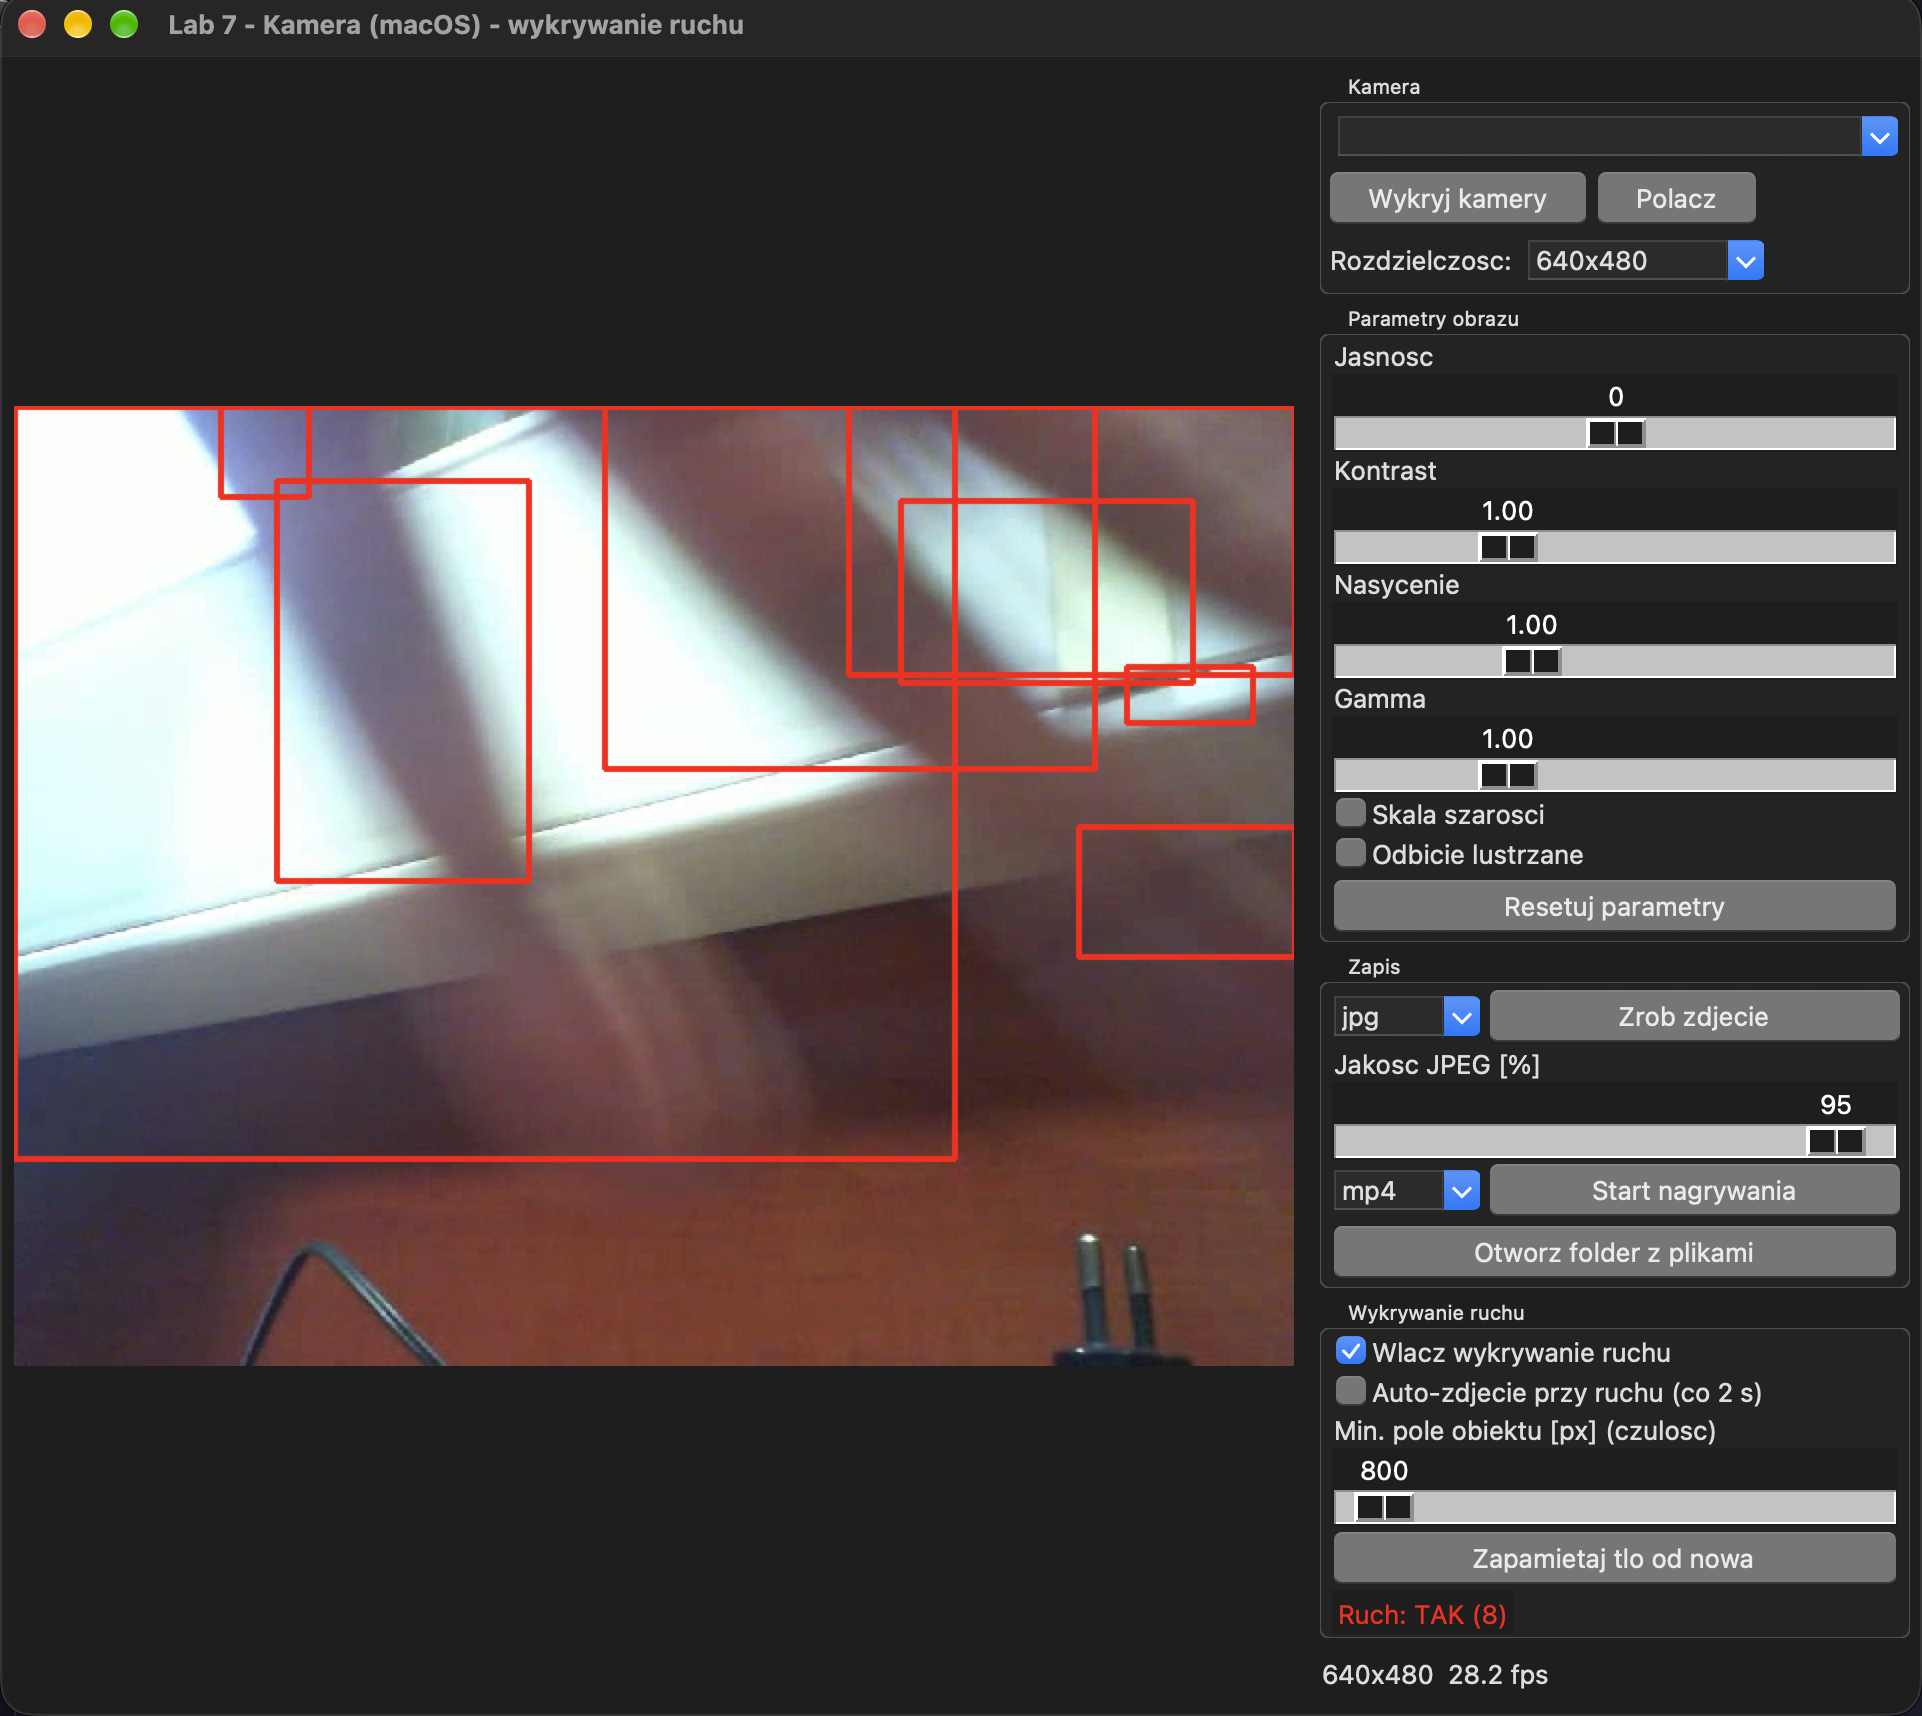
\includegraphics[width=0.8\textwidth]{ui_ruch.png}
  \caption{Okno programu \texttt{ruch\_mac.py}: podgląd z wykrytym ruchem, panel kamery, parametry
  obrazu, zapis i panel wykrywania ruchu (źródłem obrazu jest nagranie z kamery USB2.0 Camera)}
  \label{fig:okno}
\end{figure}

\subsection{Nagrane filmy}
Podczas ćwiczenia nagrano dwa filmy (tabela~\ref{tab:filmy}). Oba pliki zostały rozpoznane przez
system jako MPEG-4 Video i otwierają się w standardowych odtwarzaczach. Czas trwania wynikający
z liczby klatek i zapisanej liczby klatek na sekundę zgadza się z czasem nagrywania.

\begin{table}[H]
  \centering
  \caption{Filmy nagrane programem}
  \label{tab:filmy}
  \footnotesize
  \begin{tabular}{llcccc}
    \toprule
    Plik & Kamera & Rozdzielczość & Klatki & Klatki/s & Czas \\
    \midrule
    \texttt{film\_20261123\_084506\_652.mp4} & USB2.0 Camera & $640\times480$ & 584 & 31,1 & 18,8\,s \\
    \texttt{film\_20261123\_084552\_163.mp4} & LifeCam HD-3000 & $1280\times800$ & 292 & 10,2 & 28,5\,s \\
    \bottomrule
  \end{tabular}
\end{table}

\subsection{Zmiana parametrów obrazu}
Podczas nagrywania drugiego filmu zmieniano suwaki parametrów obrazu. Rysunek~\ref{fig:parametry}
przedstawia klatki z tego filmu przy różnych ustawieniach, a tabela~\ref{tab:parametry} średnią
jasność (składowa V w przestrzeni HSV) i średnie nasycenie (składowa S) tych klatek.

\begin{figure}[H]
  \centering
  \begin{subfigure}{0.32\textwidth}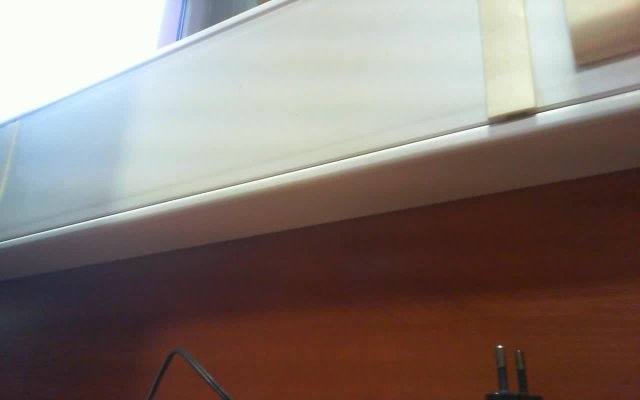
\includegraphics[width=\linewidth]{klatka_oryginal.jpg}\caption{ustawienia domyślne}\end{subfigure}\hfill
  \begin{subfigure}{0.32\textwidth}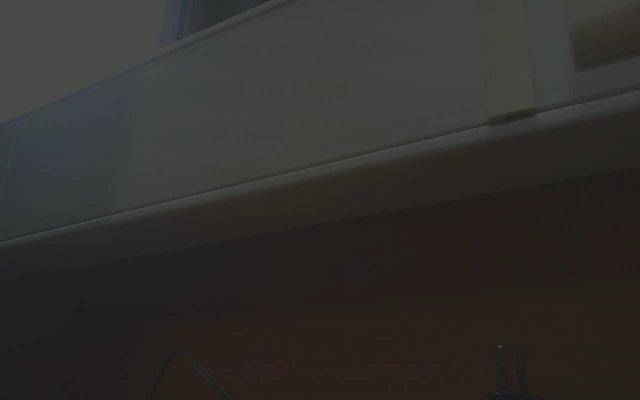
\includegraphics[width=\linewidth]{klatka_ciemno.jpg}\caption{obniżona jasność}\end{subfigure}\hfill
  \begin{subfigure}{0.32\textwidth}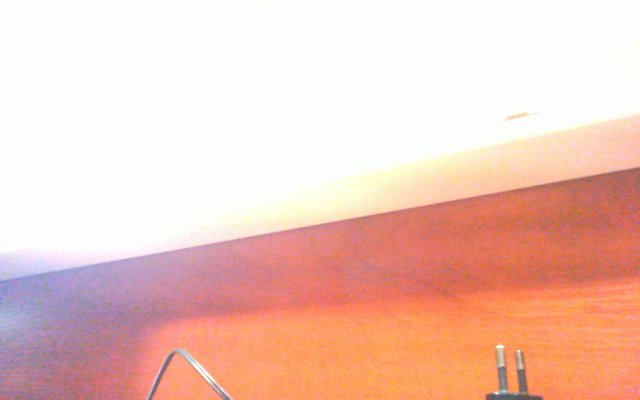
\includegraphics[width=\linewidth]{klatka_jasno.jpg}\caption{podwyższona jasność}\end{subfigure}\\[4pt]
  \begin{subfigure}{0.32\textwidth}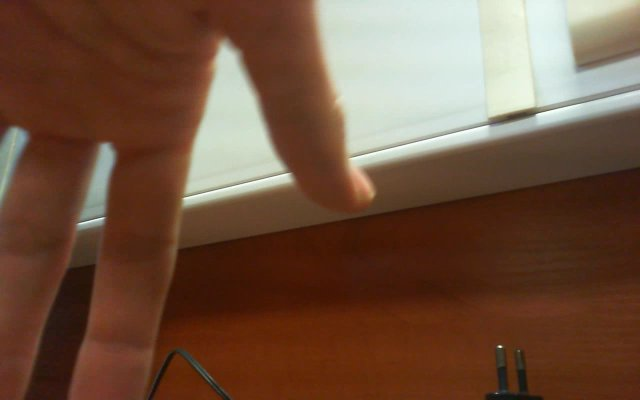
\includegraphics[width=\linewidth]{klatka_nasycenie.jpg}\caption{zwiększone nasycenie}\end{subfigure}\hspace{0.02\textwidth}
  \begin{subfigure}{0.32\textwidth}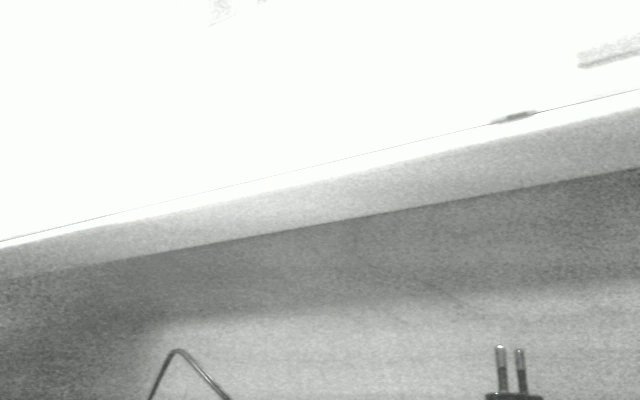
\includegraphics[width=\linewidth]{klatka_szarosc.jpg}\caption{skala szarości}\end{subfigure}
  \caption{Klatki z filmu nagranego kamerą LifeCam przy różnych parametrach obrazu}
  \label{fig:parametry}
\end{figure}

\begin{table}[H]
  \centering
  \caption{Średnia jasność i nasycenie klatek z rysunku~\ref{fig:parametry} (skala 0--255)}
  \label{tab:parametry}
  \begin{tabular}{lcc}
    \toprule
    Ustawienie & Jasność V & Nasycenie S \\
    \midrule
    domyślne & 139 & 85 \\
    obniżona jasność & 51 & 40 \\
    podwyższona jasność & 241 & 62 \\
    zwiększone nasycenie & 115 & 148 \\
    skala szarości & 200 & 4 \\
    \bottomrule
  \end{tabular}
\end{table}

\subsection{Wykrywanie ruchu}
Wykrywanie ruchu sprawdzono, przesuwając rękę przed kamerą USB2.0 Camera podczas nagrywania
pierwszego filmu. Ponieważ prostokąty nie są zapisywane do pliku, kolejne etapy algorytmu pokazano,
przetwarzając ten film klasą \texttt{MotionDetector} z ustawieniami domyślnymi
(rysunek~\ref{fig:etapy}, klatka 257, czyli 8,3\,s filmu). W tej klatce różnica z tłem osiągnęła
137 (próg 25), maska ruchu objęła 47\,\% obrazu, a program wykrył 3 obiekty. W całym filmie ruch
wykryto w 140 z 584 klatek; przed pojawieniem się ręki i po jej zniknięciu program nie zgłaszał
ruchu.

\begin{figure}[H]
  \centering
  \begin{subfigure}{0.45\textwidth}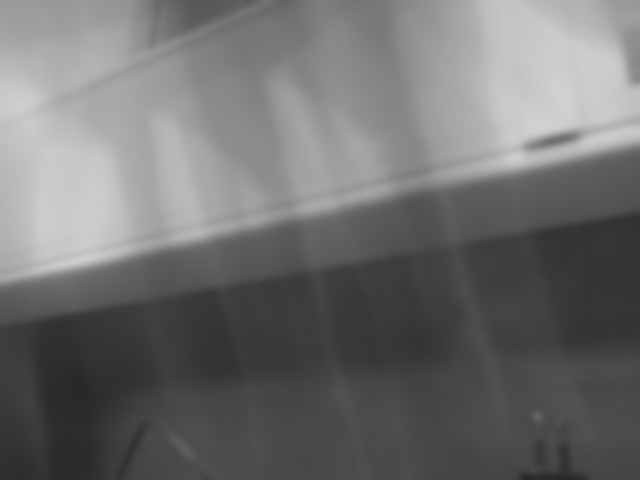
\includegraphics[width=\linewidth]{ruch_a_tlo.jpg}\caption{model tła $B$}\end{subfigure}\hfill
  \begin{subfigure}{0.45\textwidth}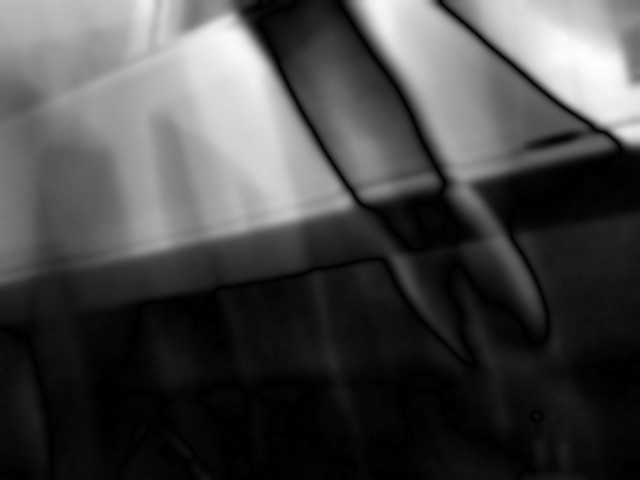
\includegraphics[width=\linewidth]{ruch_b_roznica.jpg}\caption{różnica $|I_t - B|$ (wzmocniona)}\end{subfigure}\\[4pt]
  \begin{subfigure}{0.45\textwidth}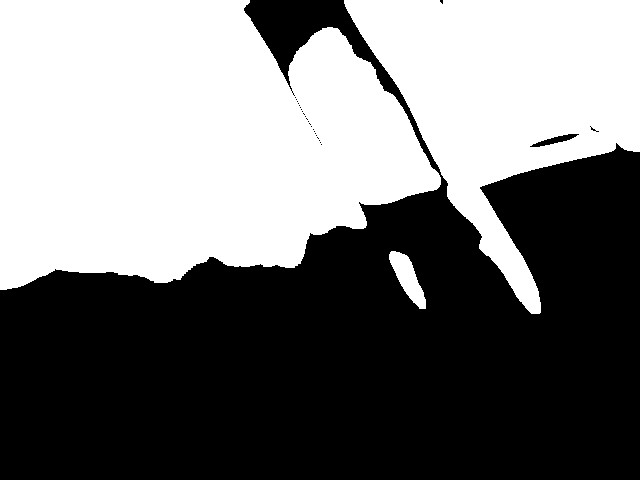
\includegraphics[width=\linewidth]{ruch_c_maska.jpg}\caption{maska po progowaniu i dylatacji}\end{subfigure}\hfill
  \begin{subfigure}{0.45\textwidth}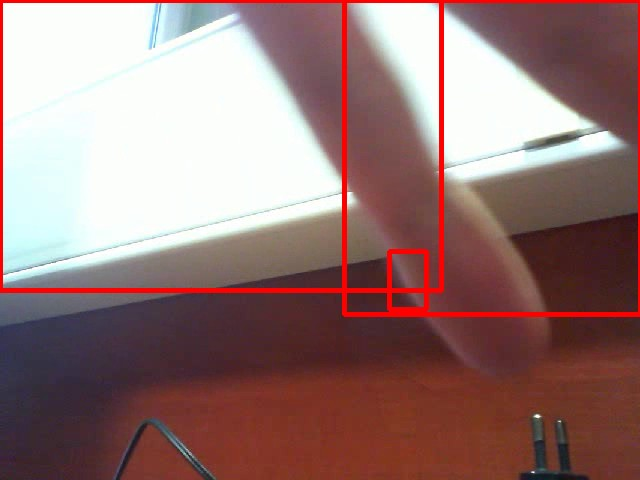
\includegraphics[width=\linewidth]{ruch_d_wynik.jpg}\caption{wykryte obiekty}\end{subfigure}
  \caption{Etapy wykrywania ruchu dla klatki z ręką przesuwaną przed kamerą}
  \label{fig:etapy}
\end{figure}

\section{Analiza wyników}
\begin{itemize}
  \item \textbf{Wybór kamery.} Nazwy kamer na liście pochodzą z AVFoundation, a ich kolejność
    zgadza się z indeksami OpenCV. Potwierdza to rozmiar pierwszej klatki po połączeniu: kamera
    USB2.0 Camera dała klatkę $640\times480$, a LifeCam $1280\times720$, czyli formaty dostępne tylko
    w danej kamerze. Kamera Megapixel nie podaje nazwy producenta, dlatego system pokazuje ją jako
    \texttt{USB2.0 Camera}.
  \item \textbf{Jakość kamery.} Wszystkie rozdzielczości z listy dały klatki o wybranym rozmiarze
    (tabela~\ref{tab:rozdz}). Lista zawiera tylko formaty zgłaszane przez kamerę, więc nie można
    wybrać rozdzielczości, której kamera nie obsługuje. Rozdzielczość zmienia format pracy samej
    kamery, a nie skaluje obrazu programowo.
  \item \textbf{Liczba klatek na sekundę.} Kamera LifeCam przy $1280\times720$ dawała około 30
    klatek/s, a przy $1280\times800$ tylko 10,2. Z zależności (2) strumień nieskompresowany
    $1280\times800$ przy 10 klatkach/s wymaga około 20,5\,MB/s, co mieści się w przepustowości USB 2.0
    (ok.\ 24,6\,MB/s), a przy 30 klatkach/s wymagałby 61\,MB/s. Prawdopodobnie format $1280\times800$
    jest w tej kamerze dostępny tylko bez kompresji, a $1280\times720$ z kompresją MJPEG. Kamera
    USB2.0 Camera przy $640\times480$ dawała 31 klatek/s (strumień nieskompresowany 18,4\,MB/s).
  \item \textbf{Parametry obrazu.} Pomiary w tabeli~\ref{tab:parametry} zgadzają się z kierunkiem
    zmian: obniżenie jasności zmniejszyło średnią jasność z 139 do 51, podwyższenie zwiększyło ją
    do 241, zwiększenie nasycenia podniosło średnie nasycenie z 85 do 148, a skala szarości dała
    nasycenie bliskie zeru (4; reszta to szum kompresji). Przy podwyższonej jasności nasycenie
    spadło do 62, ponieważ wiele pikseli osiągnęło wartość 255 we wszystkich kanałach i stało się
    białych. Zmiany są widoczne w zapisanym filmie, ponieważ przetwarzanie odbywa się przed zapisem.
  \item \textbf{Wykrywanie ruchu.} Ruch ręki został wykryty (rysunek~\ref{fig:etapy}), a przy
    nieruchomej scenie program nie zgłaszał ruchu. Ręka jest rozbita na kilka prostokątów, ponieważ
    palce i ich cienie tworzą osobne kontury maski. Metoda reaguje na każdą zmianę jasności, także
    na zmianę oświetlenia, automatycznej ekspozycji kamery lub suwaków parametrów obrazu. Po takiej
    zmianie należy użyć przycisku \emph{Zapamiętaj tło od nowa}.
  \item \textbf{Ograniczenia programu.} Parametry obrazu są zmieniane programowo, a nie w kamerze,
    więc nie poprawiają jakości samego pomiaru (np.\ zwiększenie jasności nie zmniejsza szumu).
    W macOS nie ma systemowego okna ustawień kamery, a AVFoundation nie udostępnia dla kamer USB
    ręcznej ekspozycji ani balansu bieli. Liczba klatek filmu jest ustalana na początku nagrywania,
    więc przy zmiennej liczbie klatek na sekundę czas filmu może się nieznacznie różnić od
    rzeczywistego.
\end{itemize}

\section{Wnioski}
\begin{enumerate}
  \item Napisany program realizuje polecenie prowadzącego: wykrywa podłączone kamery, pozwala
    wybrać kamerę i jej rozdzielczość, zmienia nasycenie oraz jasność, kontrast i gamma, wykonuje
    zdjęcia (JPEG, PNG, BMP) i nagrywa filmy (MP4, AVI) odczytywane przez standardowe programy.
  \item W systemie macOS do wyboru kamery po nazwie i do zmiany rozdzielczości potrzebne było
    AVFoundation, ponieważ OpenCV udostępnia tylko indeksy kamer i nie zmienia formatu ich pracy.
  \item Rozdzielczość i liczba klatek na sekundę kamery USB zależą od przepustowości łącza: duże
    klatki bez kompresji można przesłać tylko przy małej liczbie klatek na sekundę.
  \item Na ocenę wyższą zrealizowano wykrywanie ruchu metodą odejmowania tła. Metoda działa
    w czasie rzeczywistym i poprawnie wykryła ruch ręki, ale reaguje także na zmiany oświetlenia
    i ustawień obrazu.
\end{enumerate}

\section{Materiały uzupełniające}
\begin{itemize}
  \item OpenCV -- dokumentacja modułu \texttt{videoio} i \texttt{imgproc}:
    \url{https://docs.opencv.org/}
  \item OpenCV, kod obsługi AVFoundation w macOS (\texttt{cap\_avfoundation\_mac.mm}):
    \url{https://github.com/opencv/opencv/blob/5.x/modules/videoio/src/cap_avfoundation_mac.mm}
  \item Apple Developer, AVCaptureDevice: \url{https://developer.apple.com/documentation/avfoundation/avcapturedevice}
  \item USB Implementers Forum, USB Video Class 1.5: \url{https://www.usb.org/document-library/video-class-v15-document-set}
  \item Bayer filter -- Wikipedia: \url{https://en.wikipedia.org/wiki/Bayer_filter}
  \item PyObjC: \url{https://pyobjc.readthedocs.io/}
\end{itemize}

\end{document}
